\index{Linked list type definition}
\subsection{Type definition with diagram}
\justify
{
Types of linked list means looking structure of a linked list.\\
Types of linked list with diagram:
\begin{enumerate}
	\item Singly linked list, forward iteration only\\
	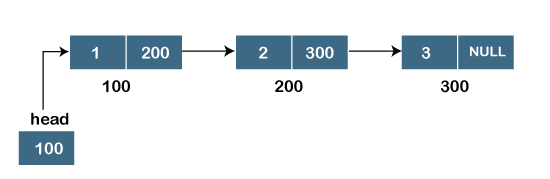
\includegraphics[scale=0.5]{Pictures/singly.png} 
	\item Double linked list, can iterate both forward and backward\\
	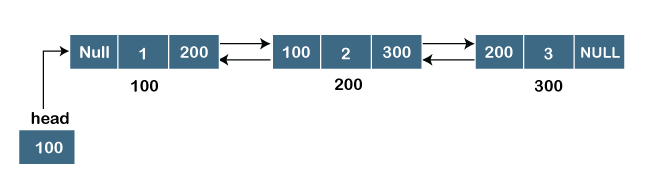
\includegraphics[scale=0.5]{Pictures/doubly.png} 
	\item Circular linked list, tail is linked with head, forward iteration only\\
	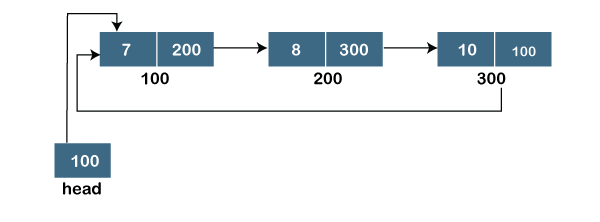
\includegraphics[scale=0.5]{Pictures/circular.png} 
	\item Double circular linked list, tail is linked with head, forward and backward both iteration supported\\
	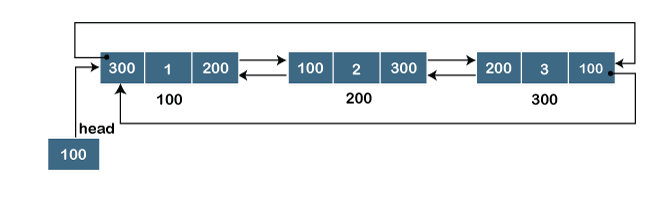
\includegraphics[scale=0.5]{Pictures/doubly circular.png}
\end{enumerate}
}
\pagebreak
\index{Algorithm to delete a node from linked list}
\subsection{Algorithm to delete a node from \enquote{pos} index}
\begin{algorithm}
\DontPrintSemicolon
\KwData{Head of the linked list and \enquote{pos} of that node which to delete.}
\KwResult{Modified list.}
\Begin
{
\If{head is null or next node of head is null and \enquote{pos} $\geq$ 1}
{
	Return null with \textcolor{red}{error} message \enquote{NullPointerException} and terminate the program.
}
Declare and initialize prev = head and curr = head.next node respectively\;
Now declare and initialize idx = 0 for loop over the linked list\;
\While{idx+1$\neq$pos and curr$\neq$null}
{
	Forward prev node one step, $prev = prev.next$\;
	Forward curr node one step, $curr = curr.next$\;
	Increment idx by 1.
}
Set prev.next node value to curr.next, $prev.next = curr.next$\;
De-allocate space for $curr$ node and free the memoey.\;
Exit with success code 0.
}
\textbf{end}

\caption{Delete a node from \enquote{pos}}
\end{algorithm}